\documentclass[10pt]{article}\usepackage[]{graphicx}\usepackage[]{xcolor}
% maxwidth is the original width if it is less than linewidth
% otherwise use linewidth (to make sure the graphics do not exceed the margin)
\makeatletter
\def\maxwidth{ %
  \ifdim\Gin@nat@width>\linewidth
    \linewidth
  \else
    \Gin@nat@width
  \fi
}
\makeatother

\definecolor{fgcolor}{rgb}{0.345, 0.345, 0.345}
\newcommand{\hlnum}[1]{\textcolor[rgb]{0.686,0.059,0.569}{#1}}%
\newcommand{\hlstr}[1]{\textcolor[rgb]{0.192,0.494,0.8}{#1}}%
\newcommand{\hlcom}[1]{\textcolor[rgb]{0.678,0.584,0.686}{\textit{#1}}}%
\newcommand{\hlopt}[1]{\textcolor[rgb]{0,0,0}{#1}}%
\newcommand{\hlstd}[1]{\textcolor[rgb]{0.345,0.345,0.345}{#1}}%
\newcommand{\hlkwa}[1]{\textcolor[rgb]{0.161,0.373,0.58}{\textbf{#1}}}%
\newcommand{\hlkwb}[1]{\textcolor[rgb]{0.69,0.353,0.396}{#1}}%
\newcommand{\hlkwc}[1]{\textcolor[rgb]{0.333,0.667,0.333}{#1}}%
\newcommand{\hlkwd}[1]{\textcolor[rgb]{0.737,0.353,0.396}{\textbf{#1}}}%
\let\hlipl\hlkwb

\usepackage{framed}
\makeatletter
\newenvironment{kframe}{%
 \def\at@end@of@kframe{}%
 \ifinner\ifhmode%
  \def\at@end@of@kframe{\end{minipage}}%
  \begin{minipage}{\columnwidth}%
 \fi\fi%
 \def\FrameCommand##1{\hskip\@totalleftmargin \hskip-\fboxsep
 \colorbox{shadecolor}{##1}\hskip-\fboxsep
     % There is no \\@totalrightmargin, so:
     \hskip-\linewidth \hskip-\@totalleftmargin \hskip\columnwidth}%
 \MakeFramed {\advance\hsize-\width
   \@totalleftmargin\z@ \linewidth\hsize
   \@setminipage}}%
 {\par\unskip\endMakeFramed%
 \at@end@of@kframe}
\makeatother

\definecolor{shadecolor}{rgb}{.97, .97, .97}
\definecolor{messagecolor}{rgb}{0, 0, 0}
\definecolor{warningcolor}{rgb}{1, 0, 1}
\definecolor{errorcolor}{rgb}{1, 0, 0}
\newenvironment{knitrout}{}{} % an empty environment to be redefined in TeX

\usepackage{alltt}
\usepackage[english]{babel}
\usepackage{graphicx,color,alltt}
\usepackage{hyperref}
\usepackage{apacite}

\setlength{\parskip}{0.5ex plus0.1ex minus0.1ex}
\setlength{\parindent}{0em}


\hypersetup{%
hyperindex,%
colorlinks,%
linktocpage,%
plainpages=false,%
linkcolor=blue,%
citecolor=blue,%
urlcolor=red,%
pdfstartview=Fit,%
pdfview={XYZ null null null}%
}
\IfFileExists{upquote.sty}{\usepackage{upquote}}{}
\begin{document}

%\SweaveOpts{concordance=TRUE}
%\SweaveOpts{engine=R,eps=FALSE}
%\SweaveOpts{keep.source=TRUE}

%\VignetteIndexEntry{lsttheory: An \textsf{R}  Package for Fast Computation of State Trait Models}
%\VignetteDepends{lsttheory}
%\VignetteKeywords{states, traits, reliability, occasion specificity, consistency}
%\VignettePackage{lsttheory}


\title{\texttt{lsttheory}: An \textsf{R}  Package for Fast Computation of State Trait Models}

\author{
  Axel Mayer\\
  Bielefeld University
}

\date{\today}
\maketitle

\begin{abstract}
This \textsf{R} \cite{RCoreTeam} package is a supplement for the article 'A Theory of States and Traits -- Revised' (SMGC; Steyer, Mayer, Geiser, \& Cole, in press). It is based on the structural equation modeling \textsf{R} package \texttt{lavaan} (Rosseel, 2012) and provides a convenient interface to compute some common models of the revised latent state-trait theory (LST-R theory). The main function of the package allows for easy specification of multistate, multistate-singletrait, and multistate-multitrait models. It automatically generates \texttt{lavaan} syntax for these models, runs the models, and returns model estimates together with reliability, occasion specificity, and consistency coefficients for the respective models. 
\end{abstract}

\noindent
{\bf Keywords:} states, traits, reliability, occasion specificity, consistency \\


\textbf{Cautionary Note:} The package is currently under development and some things may change in the future. We are at an early stage of development and it is likely that the structure and key aspects of the two packages will change. We also plan to release the package on CRAN, once we are a bit furhter in the develpment process. Please report any bugs.




\newpage
\tableofcontents

\newpage



\section{Introduction} \label{sec:intro}

\texttt{lsttheory} allows for easy specification of multistate, multistate-singletrait, and multistate-multitrait models. This vignette is structured as follows: We first describe the installation process in detail for nonexperienced users of \textsf{R}. Users who are familiar with package installation from local .zip files or from source (via Github) may wish to skip this section. We then present various kinds of LST-R theory models with syntax and model results.



\section{Installation}

The \textsf{R} package \texttt{lsttheory} can be installed from a local file. Therefore, we need to install the dependencies first. The installation has been tested under Windows 7 and under Linux (Ubuntu 11.10). It should also work under Mac OS X but we haven't tested it yet. Please make sure that you are using R version 3.0.1 or higher.

\subsection{Windows Installation}

For a Windows installation (without Rtools) we suggest installing the dependencies from a CRAN mirror first by executing
%
\begin{knitrout}
\definecolor{shadecolor}{rgb}{0.969, 0.969, 0.969}\color{fgcolor}\begin{kframe}
\begin{alltt}
\hlkwd{install.packages}\hlstd{(}\hlstr{"lavaan"}\hlstd{)}  \hlcom{## for lsttheory}
\hlkwd{install.packages}\hlstd{(}\hlstr{"shiny"}\hlstd{)}  \hlcom{## for user Interface}
\hlkwd{install.packages}\hlstd{(}\hlstr{"semPlot"}\hlstd{)}  \hlcom{## for plots}
\end{alltt}
\end{kframe}
\end{knitrout}
%
in the console and then selecting a mirror next to you. After that, the \textsf{R} package \texttt{lsttheory} can be installed using the Windows binary file (with file ending .zip) as follows:
%
\begin{knitrout}
\definecolor{shadecolor}{rgb}{0.969, 0.969, 0.969}\color{fgcolor}\begin{kframe}
\begin{alltt}
\hlkwd{install.packages}\hlstd{(}\hlstr{"D:/workspace/lsttheory_0.1-1.zip"}\hlstd{)}
\end{alltt}
\end{kframe}
\end{knitrout}
%
Please adjust the file path and version number accordingly. 

\subsection{Linux Installation}

We assume that Linux users are familiar with installing \textsf{R} packages from source. The source files is \texttt{lsttheory\_0.1-1.tar.gz} and can be downloaded from GitHub. 

\subsection{Loading the Package}

After having succesfully installed the package, we need to load them:
%
\begin{knitrout}
\definecolor{shadecolor}{rgb}{0.969, 0.969, 0.969}\color{fgcolor}\begin{kframe}
\begin{alltt}
\hlkwd{library}\hlstd{(}\hlstr{"lsttheory"}\hlstd{)}
\end{alltt}


{\ttfamily\noindent\itshape\color{messagecolor}{\#\# Lade nötiges Paket: lavaan}}

{\ttfamily\noindent\itshape\color{messagecolor}{\#\# This is lavaan 0.6-15\\\#\# lavaan is FREE software! Please report any bugs.}}\end{kframe}
\end{knitrout}
%

\newpage
\section{Multistate Models}

The lsttheory pacakge contains several simulated example datasets. The first one that we use is the dataset \texttt{d_multistate}. It contains 4 manifest variables $Y_{it}$, where the index refers to the $i$th manifest variable assessed at occasion $t$. This dataset has been used in Supplement C of Steyer, Mayer, Geiser \& Cole (in press) to describe software input for \texttt{lavaan} for LST-R models.
%
\begin{knitrout}
\definecolor{shadecolor}{rgb}{0.969, 0.969, 0.969}\color{fgcolor}\begin{kframe}
\begin{alltt}
\hlkwd{data}\hlstd{(d_multistate)}
\hlkwd{head}\hlstd{(}\hlkwd{round}\hlstd{(d_multistate,}\hlnum{2}\hlstd{))}
\end{alltt}
\begin{verbatim}
##     y11   y21   y12   y22
## 1  3.03  3.76  4.15  5.26
## 2 -1.95 -1.11 -1.99 -0.52
## 3  0.94  0.53  1.10  1.85
## 4  2.44  2.45  1.36  2.03
## 5  3.72  3.59  0.33  1.56
## 6  3.16  3.64  2.25  2.79
\end{verbatim}
\end{kframe}
\end{knitrout}
%

\subsection{Multistate Model with $\eta_t$-Congenericity}

First, we use this dataset to fit a multistate model with $\eta_t$-congenericity and conditional mean independence (see Box 4.1 of SMGC). The main function of our package to be called by the user is \texttt{lsttheory}. See \texttt{?lsttheory} for details. It is used to fit all models. The multistate model with $\eta_t$-congenericity can be specified as follows:


%
\begin{knitrout}
\definecolor{shadecolor}{rgb}{0.969, 0.969, 0.969}\color{fgcolor}\begin{kframe}
\begin{alltt}
\hlstd{m1} \hlkwb{<-} \hlkwd{lsttheory}\hlstd{(}\hlkwc{neta}\hlstd{=}\hlnum{2}\hlstd{,} \hlkwc{data}\hlstd{=d_multistate)}
\hlkwd{print}\hlstd{(m1)}
\end{alltt}
\begin{verbatim}
## 
##  Multistate Model 
##  
##     rely spey cony
## y11 0.92   NA   NA
## y21 0.92   NA   NA
## y12 0.93   NA   NA
## y22 0.91   NA   NA
## 
## 
\end{verbatim}
\end{kframe}
\end{knitrout}
%

The lsttheory function just requires two mandatory arguments: The number of common state variables $\eta_t$ and the dataset to use. In the current version of our package, the dataset may only include the manifest variables $Y_{it}$ and these should be ordered by occasion $t$ and indicator $i$, i.e., $Y_{11}, Y_{21}, \ldots, Y_{12}, Y_{22}, \ldots, Y_{13}, Y_{23}, \ldots$. The lsttheory function returns an object of class lsttheory for which several methods are available. \texttt{print(m1)} shows reliability, occasion specificity, and consistency coefficients (see Box 3.1 of SMGC). For the multistate model only reliability coefficients are available, because traits are not modeled.

The function lsttheory has automatically generated lavaan input syntax:
%
\begin{knitrout}
\definecolor{shadecolor}{rgb}{0.969, 0.969, 0.969}\color{fgcolor}\begin{kframe}
\begin{alltt}
\hlkwd{cat}\hlstd{(m1}\hlopt{@}\hlkwc{lavaansyntax}\hlstd{)}
\end{alltt}
\begin{verbatim}
## eta1 =~ 1*y11
## eta1 =~ la211*y21
## eta2 =~ 1*y12
## eta2 =~ la221*y22
## y11 ~ 0*1
## y21 ~ la210*1
## y12 ~ 0*1
## y22 ~ la220*1
## eta1 ~ ga10*1
## eta2 ~ ga20*1
## y11 ~~ eps11*y11
## y21 ~~ eps21*y21
## y12 ~~ eps12*y12
## y22 ~~ eps22*y22
## eta1 ~~ psi1*eta1
## eta2 ~~ psi2*eta2
## 
## 
## 
## 
## vareta1 := psi1
## vareta2 := psi2
## vary11 := 1^2 * vareta1 + eps11
## vary21 := la211^2 * vareta1 + eps21
## vary12 := 1^2 * vareta2 + eps12
## vary22 := la221^2 * vareta2 + eps22
## rely11 := 1^2 * vareta1 / vary11
## rely21 := la211^2 * vareta1 / vary21
## rely12 := 1^2 * vareta2 / vary12
## rely22 := la221^2 * vareta2 / vary22
\end{verbatim}
\end{kframe}
\end{knitrout}
%
and the lavaan output can be seen by calling:
%
\begin{knitrout}
\definecolor{shadecolor}{rgb}{0.969, 0.969, 0.969}\color{fgcolor}\begin{kframe}
\begin{alltt}
\hlkwd{summary}\hlstd{(m1}\hlopt{@}\hlkwc{lavaanres}\hlstd{)}
\end{alltt}
\begin{verbatim}
## lavaan 0.6.15 ended normally after 42 iterations
## 
##   Estimator                                         ML
##   Optimization method                           NLMINB
##   Number of model parameters                        13
## 
##   Number of observations                           400
## 
## Model Test User Model:
##                                                       
##   Test statistic                                 0.894
##   Degrees of freedom                                 1
##   P-value (Chi-square)                           0.344
## 
## Parameter Estimates:
## 
##   Standard errors                             Standard
##   Information                                 Expected
##   Information saturated (h1) model          Structured
## 
## Latent Variables:
##                    Estimate  Std.Err  z-value  P(>|z|)
##   eta1 =~                                             
##     y11               1.000                           
##     y21     (l211)    0.968    0.030   32.385    0.000
##   eta2 =~                                             
##     y12               1.000                           
##     y22     (l221)    0.952    0.029   33.020    0.000
## 
## Covariances:
##                    Estimate  Std.Err  z-value  P(>|z|)
##   eta1 ~~                                             
##     eta2              2.240    0.208   10.794    0.000
## 
## Intercepts:
##                    Estimate  Std.Err  z-value  P(>|z|)
##    .y11               0.000                           
##    .y21     (l210)    0.518    0.038   13.504    0.000
##    .y12               0.000                           
##    .y22     (l220)    0.732    0.045   16.215    0.000
##     eta1    (ga10)    0.466    0.092    5.076    0.000
##     eta2    (ga20)    0.952    0.095    9.989    0.000
## 
## Variances:
##                    Estimate  Std.Err  z-value  P(>|z|)
##    .y11     (ep11)    0.261    0.074    3.527    0.000
##    .y21     (ep21)    0.265    0.070    3.792    0.000
##    .y12     (ep12)    0.254    0.079    3.226    0.001
##    .y22     (ep22)    0.285    0.072    3.941    0.000
##     eta1    (psi1)    3.103    0.248   12.523    0.000
##     eta2    (psi2)    3.380    0.268   12.633    0.000
## 
## Defined Parameters:
##                    Estimate  Std.Err  z-value  P(>|z|)
##     vareta1           3.103    0.248   12.523    0.000
##     vareta2           3.380    0.268   12.633    0.000
##     vary11            3.365    0.238   14.142    0.000
##     vary21            3.176    0.225   14.142    0.000
##     vary12            3.634    0.257   14.142    0.000
##     vary22            3.347    0.237   14.142    0.000
##     rely11            0.922    0.023   40.825    0.000
##     rely21            0.917    0.023   40.472    0.000
##     rely12            0.930    0.022   42.008    0.000
##     rely22            0.915    0.022   41.052    0.000
\end{verbatim}
\end{kframe}
\end{knitrout}
%
The slot lavaanres in the m1 object contains the fitted lavaan object of class lavaan. See \texttt{?"lavaan-class"} for more information and available methods.


\subsection{Multistate Model with Essential $\eta_t$-Equivalence}

The default setting of the lsttheory function is to assume $\eta_t$-congenericity. If we want to assume essential $\eta_t$-equivalence, we need to specify an additional argument, namely the \texttt{equiv.assumption} argument, which is a list of equivalence assumptions. For the multistate model, the theta argument will be ignored. By specifying \texttt{tau="ess"}, we assume essential $\eta_t$-equivalence:
%
\begin{knitrout}
\definecolor{shadecolor}{rgb}{0.969, 0.969, 0.969}\color{fgcolor}\begin{kframe}
\begin{alltt}
\hlstd{m1} \hlkwb{<-} \hlkwd{lsttheory}\hlstd{(}\hlkwc{neta}\hlstd{=}\hlnum{2}\hlstd{,} \hlkwc{data}\hlstd{=d_multistate,}
                \hlkwc{equiv.assumption}\hlstd{=}\hlkwd{list}\hlstd{(}\hlkwc{tau}\hlstd{=}\hlstr{"ess"}\hlstd{,} \hlkwc{theta}\hlstd{=}\hlstr{"equi"}\hlstd{))}
\hlkwd{coef}\hlstd{(m1}\hlopt{@}\hlkwc{lavaanres}\hlstd{,} \hlkwc{type}\hlstd{=}\hlstr{"user"}\hlstd{)}
\end{alltt}
\begin{verbatim}
##  eta1=~y11  eta1=~y21  eta2=~y12  eta2=~y22      y11~1      la210      y12~1 
##      1.000      1.000      1.000      1.000      0.000      0.503      0.000 
##      la220       ga10       ga20      eps11      eps21      eps12      eps22 
##      0.687      0.466      0.952      0.313      0.217      0.343      0.204 
##       psi1       psi2 eta1~~eta2    vareta1    vareta2     vary11     vary21 
##      2.997      3.198      2.132      2.997      3.198      3.310      3.214 
##     vary12     vary22     rely11     rely21     rely12     rely22 
##      3.541      3.402      0.906      0.933      0.903      0.940
\end{verbatim}
\end{kframe}
\end{knitrout}
%



\subsection{Multistate Model with $\eta_t$-Equivalence}

Similarly, if we want to assume $\eta_t$-equivalence, we specify the equivalence assumption as follows:
%
\begin{knitrout}
\definecolor{shadecolor}{rgb}{0.969, 0.969, 0.969}\color{fgcolor}\begin{kframe}
\begin{alltt}
\hlstd{m1} \hlkwb{<-} \hlkwd{lsttheory}\hlstd{(}\hlkwc{neta}\hlstd{=}\hlnum{2}\hlstd{,} \hlkwc{data}\hlstd{=d_multistate,}
                \hlkwc{equiv.assumption}\hlstd{=}\hlkwd{list}\hlstd{(}\hlkwc{tau}\hlstd{=}\hlstr{"equi"}\hlstd{,} \hlkwc{theta}\hlstd{=}\hlstr{"equi"}\hlstd{))}
\hlkwd{coef}\hlstd{(m1}\hlopt{@}\hlkwc{lavaanres}\hlstd{,} \hlkwc{type}\hlstd{=}\hlstr{"user"}\hlstd{)}
\end{alltt}
\begin{verbatim}
##  eta1=~y11  eta1=~y21  eta2=~y12  eta2=~y22      y11~1      y21~1      y12~1 
##      1.000      1.000      1.000      1.000      0.000      0.000      0.000 
##      y22~1       ga10       ga20      eps11      eps21      eps12      eps22 
##      0.000      0.762      1.383      0.462      0.320      0.639      0.379 
##       psi1       psi2 eta1~~eta2    vareta1    vareta2     vary11     vary21 
##      2.936      3.088      2.132      2.936      3.088      3.398      3.256 
##     vary12     vary22     rely11     rely21     rely12     rely22 
##      3.727      3.467      0.864      0.902      0.829      0.891
\end{verbatim}
\end{kframe}
\end{knitrout}
%



\subsection{Multistate Models with Scale Invariance}

In order to add scale invariance assumptions over time, we need to specify the scale.invariance argument. The default is not to assume scale invariance. The scale invariance argument is a list of four entries. For the multistate models, only the first and the second entry are relevant. The first entry refers to scale invariance of intercepts and the second entry refers to scale invariance of loadings. For example, if we want to specify a multistate model with $\eta_t$-congenericity and scale invariance of intercepts and loadings, the function call is:

%
\begin{knitrout}
\definecolor{shadecolor}{rgb}{0.969, 0.969, 0.969}\color{fgcolor}\begin{kframe}
\begin{alltt}
\hlstd{m1} \hlkwb{<-} \hlkwd{lsttheory}\hlstd{(}\hlkwc{neta}\hlstd{=}\hlnum{2}\hlstd{,} \hlkwc{data}\hlstd{=d_multistate,}
                \hlkwc{scale.invariance}\hlstd{=}\hlkwd{list}\hlstd{(}\hlkwc{lait0}\hlstd{=}\hlnum{TRUE}\hlstd{,} \hlkwc{lait1}\hlstd{=}\hlnum{TRUE}\hlstd{,} \hlkwc{lat0}\hlstd{=}\hlnum{TRUE}\hlstd{,} \hlkwc{lat1}\hlstd{=}\hlnum{TRUE}\hlstd{))}
\hlkwd{coef}\hlstd{(m1}\hlopt{@}\hlkwc{lavaanres}\hlstd{,} \hlkwc{type}\hlstd{=}\hlstr{"user"}\hlstd{)}
\end{alltt}
\begin{verbatim}
##  eta1=~y11      la211  eta2=~y12      la211      y11~1      la210      y12~1 
##      1.000      0.979      1.000      0.979      0.000      0.608      0.000 
##      la210       ga10       ga20      eps11      eps21      eps12      eps22 
##      0.608      0.415      1.007      0.282      0.254      0.310      0.243 
##       psi1       psi2 eta1~~eta2    vareta1    vareta2     vary11     vary21 
##      3.068      3.280      2.194      3.068      3.280      3.350      3.193 
##     vary12     vary22     rely11     rely21     rely12     rely22 .p2.==.p4. 
##      3.590      3.385      0.916      0.920      0.914      0.928      0.000 
## .p6.==.p8. 
##      0.000
\end{verbatim}
\end{kframe}
\end{knitrout}
%
Of course, the scale invariance argument can also be used for a multistate model with essential $\eta_t$-equivalence. Then, the lait1 entry is ignored.
%
\begin{knitrout}
\definecolor{shadecolor}{rgb}{0.969, 0.969, 0.969}\color{fgcolor}\begin{kframe}
\begin{alltt}
\hlstd{m1} \hlkwb{<-} \hlkwd{lsttheory}\hlstd{(}\hlkwc{neta}\hlstd{=}\hlnum{2}\hlstd{,} \hlkwc{data}\hlstd{=d_multistate,} \hlkwc{equiv.assumption}\hlstd{=}\hlkwd{list}\hlstd{(}\hlkwc{tau}\hlstd{=}\hlstr{"ess"}\hlstd{,} \hlkwc{theta}\hlstd{=}\hlstr{"equi"}\hlstd{),} \hlkwc{scale.invariance}\hlstd{=}\hlkwd{list}\hlstd{(}\hlkwc{lait0}\hlstd{=}\hlnum{TRUE}\hlstd{,} \hlkwc{lait1}\hlstd{=}\hlnum{TRUE}\hlstd{,} \hlkwc{lat0}\hlstd{=}\hlnum{TRUE}\hlstd{,} \hlkwc{lat1}\hlstd{=}\hlnum{TRUE}\hlstd{))}
\end{alltt}
\end{kframe}
\end{knitrout}
%
For a multistate model with $\eta_t$-equivalence, all scale invariance settings are ignored.


\newpage
\section{Multistate-Singletrait Models}

\subsection{Multistate-Singletrait Models with $\theta$-Congenericity}

The same function lsttheory can also be used to fit multistate-singletrait models in LST-R theory. We only need to specify that there is one $\theta$ variable in addition to the specification of the corresponding multistate model. The following syntax specifies a multistate-singletrait model with these assumptions:
%
\begin{itemize}
  \item $\eta_t$-congenericity (Box 4.1 of SMGC)
  \item conditional mean independence (Box 4.1 of SMGC)
  \item $\theta$-congenericity (Box 5.1 of SMGC)
\end{itemize}
%
\begin{knitrout}
\definecolor{shadecolor}{rgb}{0.969, 0.969, 0.969}\color{fgcolor}\begin{kframe}
\begin{alltt}
\hlstd{m1} \hlkwb{<-} \hlkwd{lsttheory}\hlstd{(}\hlkwc{neta}\hlstd{=}\hlnum{3}\hlstd{,} \hlkwc{ntheta}\hlstd{=}\hlnum{1}\hlstd{,} \hlkwc{data}\hlstd{=d_multistate02)}
\hlkwd{print}\hlstd{(m1)}
\end{alltt}
\begin{verbatim}
## 
##  Singletrait-Multistate Model 
##  
##     rely spey cony
## y11 0.73 0.25 0.47
## y21 0.83 0.29 0.54
## y31 0.64 0.22 0.42
## y12 0.77 0.20 0.57
## y22 0.81 0.21 0.60
## y32 0.65 0.17 0.48
## y13 0.74 0.26 0.48
## y23 0.79 0.28 0.51
## y33 0.68 0.24 0.44
## 
## 
\end{verbatim}
\end{kframe}
\end{knitrout}
%
Note that we use the \texttt{multistate02} data set for this model -- it contains three indicators at three occasions of measurement. We now also get estimates for the occasion specificity and consistency coefficents in addition to the reliability coefficients. To see all parameters of the model:
%
\begin{knitrout}
\definecolor{shadecolor}{rgb}{0.969, 0.969, 0.969}\color{fgcolor}\begin{kframe}
\begin{alltt}
\hlkwd{coef}\hlstd{(m1}\hlopt{@}\hlkwc{lavaanres}\hlstd{,} \hlkwc{type}\hlstd{=}\hlstr{"user"}\hlstd{)}
\end{alltt}
\begin{verbatim}
##    eta1=~y11        la211        la311    eta2=~y12        la221        la321 
##        1.000        1.221        0.801        1.000        1.211        0.772 
##    eta3=~y13        la231        la331        y11~1        la210        la310 
##        1.000        1.233        0.828        0.000        0.217        0.570 
##        y12~1        la220        la320        y13~1        la230        la330 
##        0.000        0.212        0.578        0.000        0.262        0.574 
##       eta1~1         ga20         ga30        eps11        eps21        eps31 
##        0.000        0.400       -0.115        1.070        0.874        1.029 
##        eps12        eps22        eps32        eps13        eps23        eps33 
##        0.932        1.036        0.956        1.028        1.146        0.944 
##         psi1         psi2         psi3 theta1=~eta1         ga21         ga31 
##        0.988        0.792        1.014        1.000        1.099        0.999 
##    vartheta1      mtheta1      vareta1      vareta2      vareta3       vary11 
##        1.857        0.611        2.845        3.035        2.869        3.914 
##       vary21       vary31       vary12       vary22       vary32       vary13 
##        5.116        2.853        3.967        5.483        2.765        3.897 
##       vary23       vary33       rely11       rely21       rely31       rely12 
##        5.511        2.912        0.727        0.829        0.639        0.765 
##       rely22       rely32       rely13       rely23       rely33       spey11 
##        0.811        0.654        0.736        0.792        0.676        0.252 
##       spey21       spey31       spey12       spey22       spey32       spey13 
##        0.288        0.222        0.200        0.212        0.171        0.260 
##       spey23       spey33       cony11       cony21       cony31       cony12 
##        0.280        0.239        0.474        0.541        0.417        0.565 
##       cony22       cony32       cony13       cony23       cony33 
##        0.599        0.483        0.476        0.512        0.437
\end{verbatim}
\end{kframe}
\end{knitrout}
%



\subsection{Multistate-Singletrait Models with $\theta$-Equivalence}

We don't show all possible combinations of assumptions. We just give one more example of a multistate-singletrait model with this set of assumptions:
%
\begin{itemize}
  \item essential $\eta_t$-equivalence (Box 4.1 of SMGC)
  \item scale invariance over time
  \item conditional mean independence (Box 4.1 of SMGC)
  \item $\theta$-equivalence (Box 5.1 of SMGC)
\end{itemize}
%
%
\begin{knitrout}
\definecolor{shadecolor}{rgb}{0.969, 0.969, 0.969}\color{fgcolor}\begin{kframe}
\begin{alltt}
\hlstd{m1} \hlkwb{<-} \hlkwd{lsttheory}\hlstd{(}\hlkwc{neta}\hlstd{=}\hlnum{3}\hlstd{,} \hlkwc{ntheta}\hlstd{=}\hlnum{1}\hlstd{,} \hlkwc{data}\hlstd{=d_multistate02,}
                \hlkwc{equiv.assumption}\hlstd{=}\hlkwd{list}\hlstd{(}\hlkwc{tau}\hlstd{=}\hlstr{"ess"}\hlstd{,} \hlkwc{theta}\hlstd{=}\hlstr{"equi"}\hlstd{),}
                \hlkwc{scale.invariance}\hlstd{=}\hlkwd{list}\hlstd{(}\hlkwc{lait0}\hlstd{=}\hlnum{TRUE}\hlstd{,} \hlkwc{lait1}\hlstd{=}\hlnum{TRUE}\hlstd{,} \hlkwc{lat0}\hlstd{=}\hlnum{TRUE}\hlstd{,} \hlkwc{lat1}\hlstd{=}\hlnum{TRUE}\hlstd{))}
\hlkwd{coef}\hlstd{(m1}\hlopt{@}\hlkwc{lavaanres}\hlstd{,} \hlkwc{type}\hlstd{=}\hlstr{"user"}\hlstd{)}
\end{alltt}
\begin{verbatim}
##    eta1=~y11    eta1=~y21    eta1=~y31    eta2=~y12    eta2=~y22    eta2=~y32 
##        1.000        1.000        1.000        1.000        1.000        1.000 
##    eta3=~y13    eta3=~y23    eta3=~y33        y11~1        la210        la310 
##        1.000        1.000        1.000        0.000        0.385        0.421 
##        y12~1        la210        la310        y13~1        la210        la310 
##        0.000        0.385        0.421        0.000        0.385        0.421 
##       eta1~1       eta2~1       eta3~1        eps11        eps21        eps31 
##        0.000        0.000        0.000        1.064        1.381        0.961 
##        eps12        eps22        eps32        eps13        eps23        eps33 
##        1.004        1.591        0.878        1.090        1.673        0.831 
##         psi1         psi2         psi3 theta1=~eta1 theta1=~eta2 theta1=~eta3 
##        0.861        0.939        0.963        1.000        1.000        1.000 
##    vartheta1      mtheta1      vareta1      vareta2      vareta3       vary11 
##        1.855        0.727        2.716        2.794        2.817        3.779 
##       vary21       vary31       vary12       vary22       vary32       vary13 
##        4.097        3.677        3.797        4.384        3.672        3.908 
##       vary23       vary33       rely11       rely21       rely31       rely12 
##        4.490        3.648        0.719        0.663        0.739        0.736 
##       rely22       rely32       rely13       rely23       rely33       spey11 
##        0.637        0.761        0.721        0.627        0.772        0.228 
##       spey21       spey31       spey12       spey22       spey32       spey13 
##        0.210        0.234        0.247        0.214        0.256        0.246 
##       spey23       spey33       cony11       cony21       cony31       cony12 
##        0.214        0.264        0.491        0.453        0.504        0.488 
##       cony22       cony32       cony13       cony23       cony33 .p11.==.p14. 
##        0.423        0.505        0.475        0.413        0.508        0.000 
## .p11.==.p17. .p12.==.p15. .p12.==.p18. 
##        0.000        0.000        0.000
\end{verbatim}
\end{kframe}
\end{knitrout}
%



\newpage
\section{Multistate-Doubletrait Models}

For the mulistate doubletrait models, we need to use a different data set, because we need at least two common state variables for each of the $\theta$ variables. The simulated data set is called \texttt{multitraitmultistate} and contains 8 manifest variables $Y_{it}$ distributed across 4 occasions of measurement:

%
\begin{knitrout}
\definecolor{shadecolor}{rgb}{0.969, 0.969, 0.969}\color{fgcolor}\begin{kframe}
\begin{alltt}
\hlkwd{data}\hlstd{(d_multitraitmultistate)}
\hlkwd{head}\hlstd{(}\hlkwd{round}\hlstd{(d_multitraitmultistate,}\hlnum{2}\hlstd{))}
\end{alltt}
\begin{verbatim}
##     y11   y21   y12   y22   y13   y23   y14   y24
## 1  1.55  1.99  0.63  0.02  1.61  2.26  4.85  3.55
## 2  1.92  3.43 -0.66 -0.58  2.81  4.27  1.58  0.97
## 3 -0.07  0.32  1.81  1.83  1.73  4.05  0.70  2.93
## 4 -0.67 -1.67  1.01  1.55 -1.79 -2.35 -0.67  0.79
## 5  0.53  0.65  0.11 -0.47 -1.10 -1.03  2.91 -0.56
## 6 -1.90 -2.47  1.46  3.04  1.02 -0.08  0.88  1.39
\end{verbatim}
\end{kframe}
\end{knitrout}
%



\subsection{Multistate-Doubletrait Models with $\theta_1,\theta_2$-Congenericity}


The first model that we want to show with this dataset is a multistate-doubletrait model with these assumptions:
%
\begin{itemize}
  \item $\eta_t$-congenericity (Box 4.1 of SMGC)
  \item conditional mean independence (Box 4.1 of SMGC)
  \item $\theta_1$-congenericity (Box 6.1 of SMGC)
  \item $\theta_2$-congenericity (Box 6.1 of SMGC)
\end{itemize}
%

The model syntax is:

%
\begin{knitrout}
\definecolor{shadecolor}{rgb}{0.969, 0.969, 0.969}\color{fgcolor}\begin{kframe}
\begin{alltt}
\hlstd{m1} \hlkwb{<-} \hlkwd{lsttheory}\hlstd{(}\hlkwc{neta}\hlstd{=}\hlnum{4}\hlstd{,} \hlkwc{ntheta}\hlstd{=}\hlnum{2}\hlstd{,} \hlkwc{data}\hlstd{=d_multitraitmultistate)}
\hlkwd{coef}\hlstd{(m1}\hlopt{@}\hlkwc{lavaanres}\hlstd{,} \hlkwc{type}\hlstd{=}\hlstr{"user"}\hlstd{)}
\end{alltt}
\begin{verbatim}
##      eta1=~y11          la211      eta2=~y12          la221      eta3=~y13 
##          1.000          1.203          1.000          1.195          1.000 
##          la231      eta4=~y14          la241          y11~1          la210 
##          1.204          1.000          1.080          0.000          0.313 
##          y12~1          la220          y13~1          la230          y14~1 
##          0.000          0.380          0.000          0.307          0.000 
##          la240         eta1~1           ga20         eta3~1           ga40 
##          0.382          0.000          0.398          0.000          0.234 
##          eps11          eps21          eps12          eps22          eps13 
##          0.941          1.020          1.136          0.857          0.915 
##          eps23          eps14          eps24           psi1           psi2 
##          1.038          0.901          1.158          0.955          1.141 
##           psi3           psi4   theta1=~eta1           ga21   theta2=~eta3 
##          1.390          0.681          1.000          0.649          1.000 
##           ga41      vartheta1      vartheta2        mtheta1        mtheta2 
##          0.858          2.694          2.580          0.450          0.928 
## theta1~~theta2        vareta1        vareta2        vareta3        vareta4 
##          1.721          3.649          2.277          3.970          2.583 
##         vary11         vary21         vary12         vary22         vary13 
##          4.590          6.303          3.413          4.106          4.885 
##         vary23         vary14         vary24         rely11         rely21 
##          6.795          3.484          4.173          0.795          0.838 
##         rely12         rely22         rely13         rely23         rely14 
##          0.667          0.791          0.813          0.847          0.741 
##         rely24         spey11         spey21         spey12         spey22 
##          0.722          0.208          0.219          0.334          0.397 
##         spey13         spey23         spey14         spey24         cony11 
##          0.284          0.297          0.196          0.191          0.587 
##         cony21         cony12         cony22         cony13         cony23 
##          0.619          0.333          0.395          0.528          0.551 
##         cony14         cony24 
##          0.546          0.532
\end{verbatim}
\end{kframe}
\end{knitrout}
%

\newpage

\section{Plot LST-R Theory Models with \texttt{semPlot}}

The package \texttt{semPlot} by Sacha Epskamp can be used to plot such LST-R models as shown in this vignette. To plot the multistate-doubletrait model shown in last section, we call:

%
\begin{knitrout}
\definecolor{shadecolor}{rgb}{0.969, 0.969, 0.969}\color{fgcolor}\begin{kframe}
\begin{alltt}
\hlkwd{library}\hlstd{(semPlot)}
\hlkwd{semPaths}\hlstd{(m1}\hlopt{@}\hlkwc{lavaanres}\hlstd{,} \hlkwc{style}\hlstd{=}\hlstr{"lisrel"}\hlstd{,} \hlkwc{intercepts}\hlstd{=F,}
         \hlkwc{layout}\hlstd{=}\hlstr{"tree2"}\hlstd{,} \hlkwc{rotation}\hlstd{=}\hlnum{4}\hlstd{,} \hlkwc{nCharNodes}\hlstd{=}\hlnum{4}\hlstd{,} \hlkwc{nCharEdges}\hlstd{=}\hlnum{4}\hlstd{,}
         \hlkwc{optimizeLatRes}\hlstd{=F,} \hlkwc{residScale}\hlstd{=}\hlnum{10}\hlstd{)}
\end{alltt}
\end{kframe}
\end{knitrout}
%

which gives the figure shown in Figure \ref{fig:semplot01}.

%
\begin{figure}
\centering
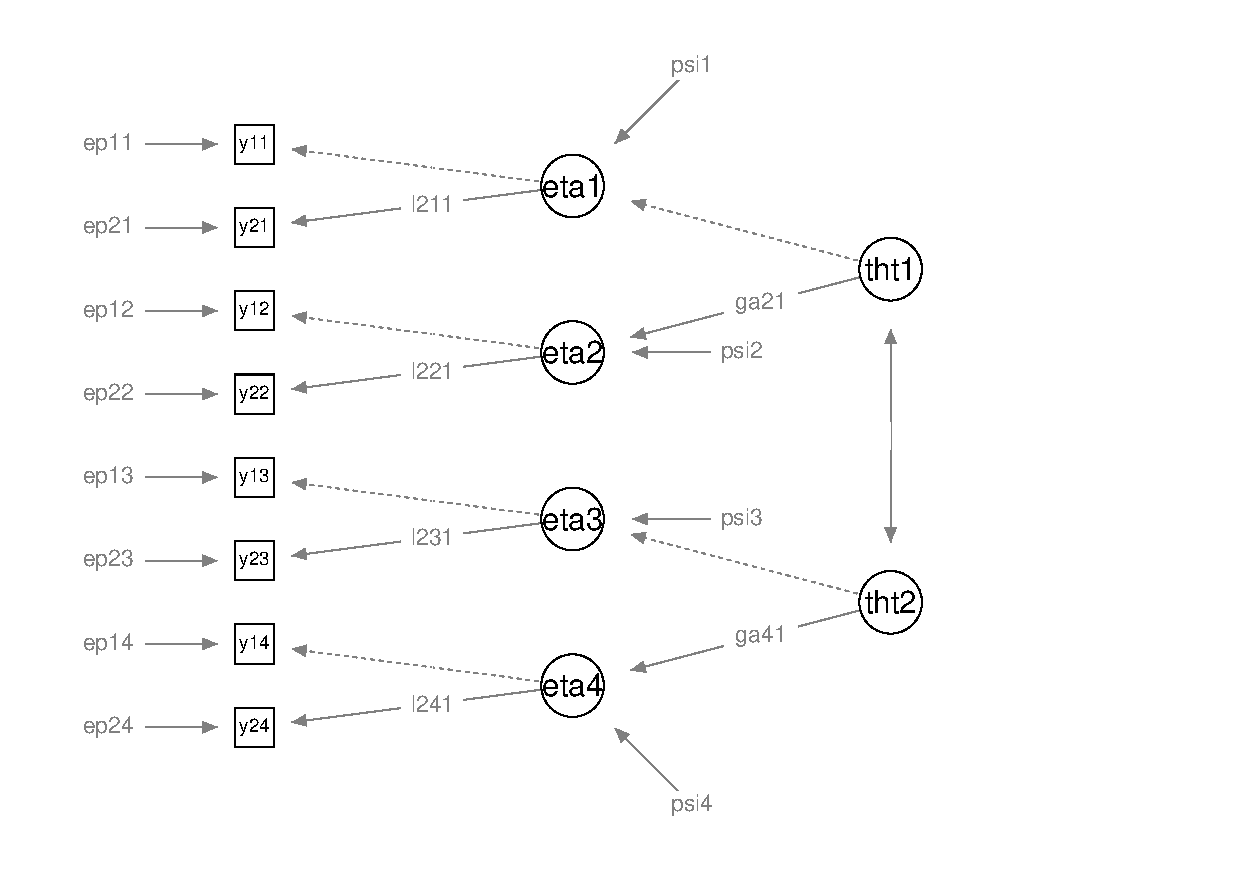
\includegraphics[scale=0.7]{semplot01}
\caption{Multistate-Doubletrait Model.}
\label{fig:semplot01}
\end{figure}
%           

\section*{References}

\begin{description}
\item Epskamp, S. (2013). semPlot: Path diagrams and visual analysis of various
  SEM packages' output. R package version 0.3.2.  \url{http://CRAN.R-project.org/package=semPlot}
\item R Core Team (2013). R: A language and environment for statistical computing.
  R Foundation for Statistical Computing, Vienna, Austria. URL \url{http://www.R-project.org/}.
\item Rosseel, Y. (2012). lavaan: An R Package for Structural Equation Modeling.
  Journal of Statistical Software, 48(2), 1--36. URL  \url{http://www.jstatsoft.org/v48/i02/}.
\item Steyer, R., Mayer, A., Geiser, C., \& Cole, D.A. (in press). A theory of states and traits -- revised. Annual Review of Clinical Psychology.
\end{description}


\end{document}
